%
% kartkugel.tex
%
% (c) 2021 Prof Dr Andreas Müller, OST Ostschweizer Fachhochschule
%
\documentclass[tikz]{standalone}
\usepackage{times}
\usepackage{amsmath}
\usepackage{txfonts}
\usepackage[utf8]{inputenc}
\usepackage{graphics}
\usetikzlibrary{arrows,intersections,math}
\usepackage{ifthen}
\begin{document}
\definecolor{kugelcolor}{rgb}{1.0,0.4,0.4}
\definecolor{kartcolor}{rgb}{0.4,0.6,1.0}
\definecolor{punktcolor}{rgb}{0.2,0.8,0.0}


\newboolean{showgrid}
\setboolean{showgrid}{false}
\def\breite{5}
\def\hoehe{5}

\begin{tikzpicture}[>=latex,thick]

% Povray Bild
\node at (0,0) {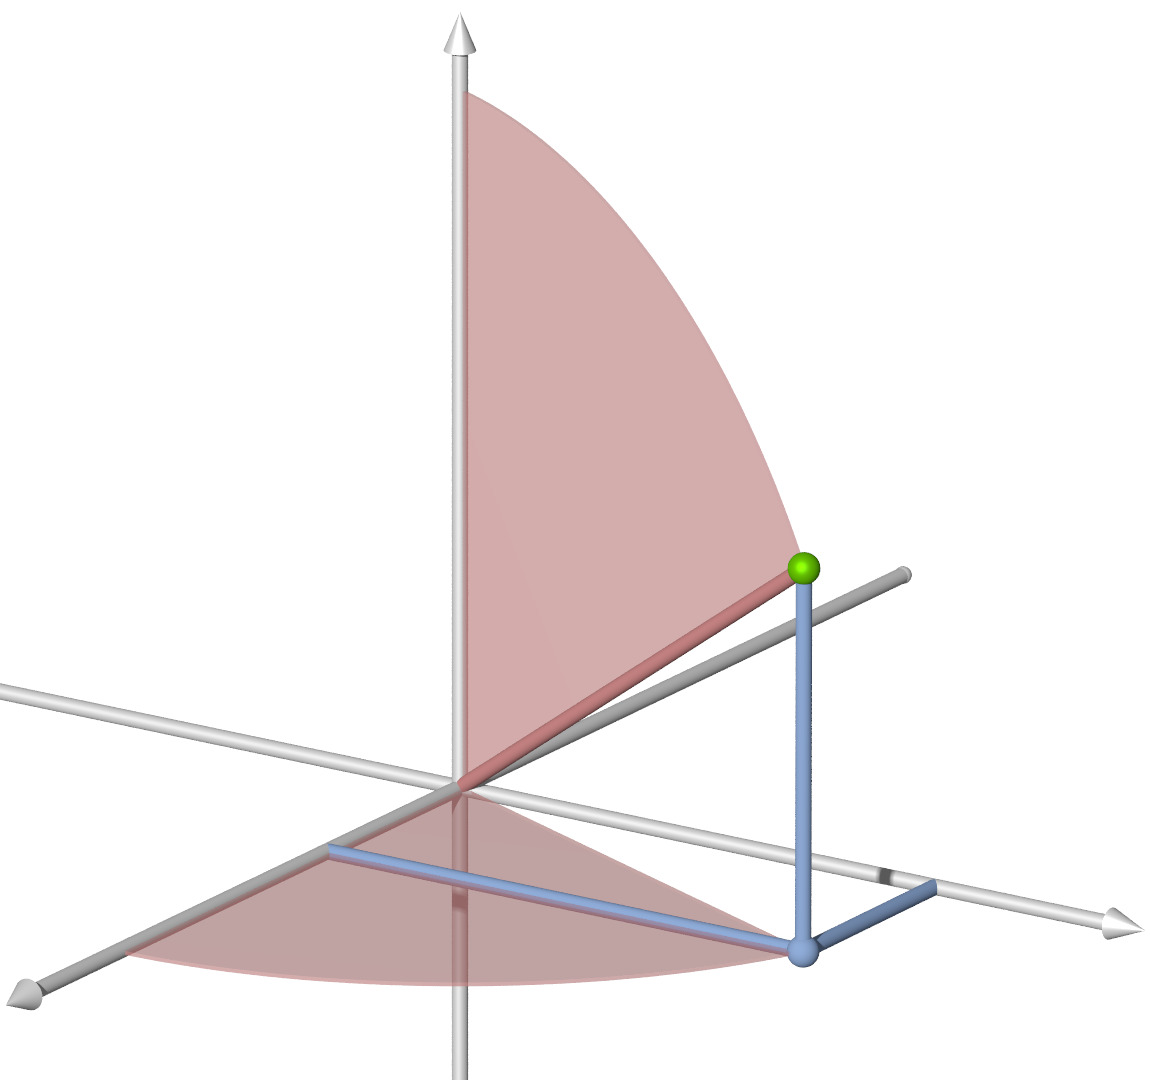
\includegraphics[width=10cm]{kartkugel.jpg}};

% Gitter
\ifthenelse{\boolean{showgrid}}{
\draw[step=0.1,line width=0.1pt] (-\breite,-\hoehe) grid (\breite, \hoehe);
\draw[step=0.5,line width=0.4pt] (-\breite,-\hoehe) grid (\breite, \hoehe);
\draw                            (-\breite,-\hoehe) grid (\breite, \hoehe);
\fill (0,0) circle[radius=0.05];
}{}

\node[color=punktcolor] at (2.3,-0.1) {$P$};

\begin{scope}[xshift=-1.0cm,yshift=-2.5cm]
	\fill[color=white,opacity=0.7] (-0.5,-0.2) rectangle ++(1.0,0.4);
	\node[color=kugelcolor] at (0,0) {$y^2=\varphi$};
\end{scope}

\begin{scope}[xshift=-0.4cm,yshift=-1.3cm]
	\fill[color=white,opacity=0.7] (-0.5,-0.2) rectangle ++(1.0,0.4);
	\node[color=kugelcolor] at (0,0) {$y^3=\vartheta$};
\end{scope}

\begin{scope}[xshift=0.9cm,yshift=-1.3cm,rotate=32]
	\fill[color=white,opacity=0.7] (-0.5,-0.2) rectangle ++(1,0.4);
	\node[color=kugelcolor] at (0,0) [rotate=32] {$y^1=r$};
\end{scope}

\node[color=kartcolor] at (-2.2,-2.4) {$x^1$};
\node[color=kartcolor] at (3.3,-2.7) {$x^2$};
\node[color=kartcolor] at (2.3,-1.7) {$x^3$};

\node at (-0.7,4.5) {$x^3$};
\node at (-4.8,-3.6) {$x^1$};
\node at (4.9,-3.0) {$x^2$};

\end{tikzpicture}

\end{document}

